\documentclass[main.tex]{subfiles}
\begin{document}
    \section{Frame}
   	 The ladder frame is the design that the team decided to go with, similar to the frame for Competition 2 design. It consists of two L-Beams facing towards each other with four I-Beam cross beams connecting them. There are a few major design changes that were made to adapt to changes in the pod subsystems. A longer frame was vital in the new design to accommodate the new friction drive propulsion system and the longer Eddy Current brakes. In addition, to avoid excessive torsional forces, as well as to simplify mounting of the friction drive and the shell, the frame was made narrower. For battery mounting, a flat plate was added parallel to the I-Beams. This flat plate is also vital for reducing deformities from the transverse forces of the EC Brakes.\\

    An investigation was conducted to assess the feasibility of  a honeycomb plate with sections cut out as the frame. While this design would reduce overall mass, there are three major factors which made this design infeasible. Firstly, a custom made honeycomb plate would have broken the philosophy of modularity for the Waterloop pod: if any parts needed to be modified, new holes would have to be cut into the honeycomb structure. Secondly, the honeycomb plate would have been around \$4000, about twice as expensive as the ladder frame design. Finally, due to the complex shape of the  composite, the honeycomb’s performance under load is difficult to analyze and simulate correctly, and after some attempts it was decided that there is insufficient technical expertise in the team to verify the feasibility of this design. For future competitions, we may reconsider the honeycomb frame.\\

    The materials used in the frame are 7075-T6 for the I-beam cross-members and 6061-T6 for the L-Beams. Originally, the entire frame was to use 6061-T6, like the Competition 2 design, but due to extreme forces from the Eddy Current Brakes, the material had to be changed to 7075-T6 on the I-Beams to achieve a safety factor of 4.176 when the brakes activate. For the L-beams, 6061 T6 will be structurally sufficient and much less expensive.

    \subsection{Overall Design}
    \begin{figure}
        \centering
        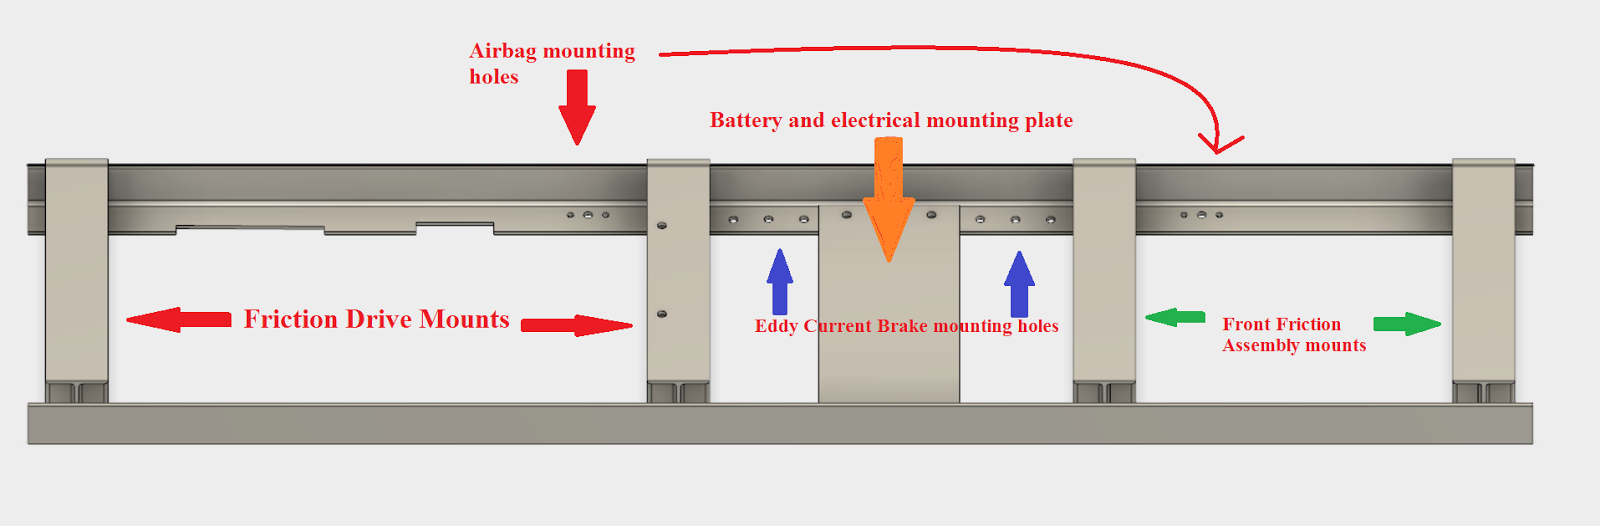
\includegraphics[width=\linewidth]{images/fig24}
        \caption{Frame Design}
        \label{fig:frame-design}
    \end{figure}
    \begin{itemize}
        \item The mass of the whole frame will be approximately 25 kg
        \item Dimensions would be 2.1m x 0.44m
    \end{itemize}
    Full cost breakdown, comments on manufacturability and production costs\\
    “A full Bill of Materials can be found in Appendix E.”

    \subsection{Structural}
    The first 4 modes of vibration of this design accounting for subsystem weights and forces are as follows:
    \begin{enumerate}
    	\item 94.81Hz
    	\item 94.83 Hz
    	\item 96.6 Hz
    	\item 125.7 Hz
    \end{enumerate}
	To dampen the vibrations of the Friction Drive, there are 4 airbags installed directly to the frame that act as a suspension system.\\
    \begin{figure}
        \centering
        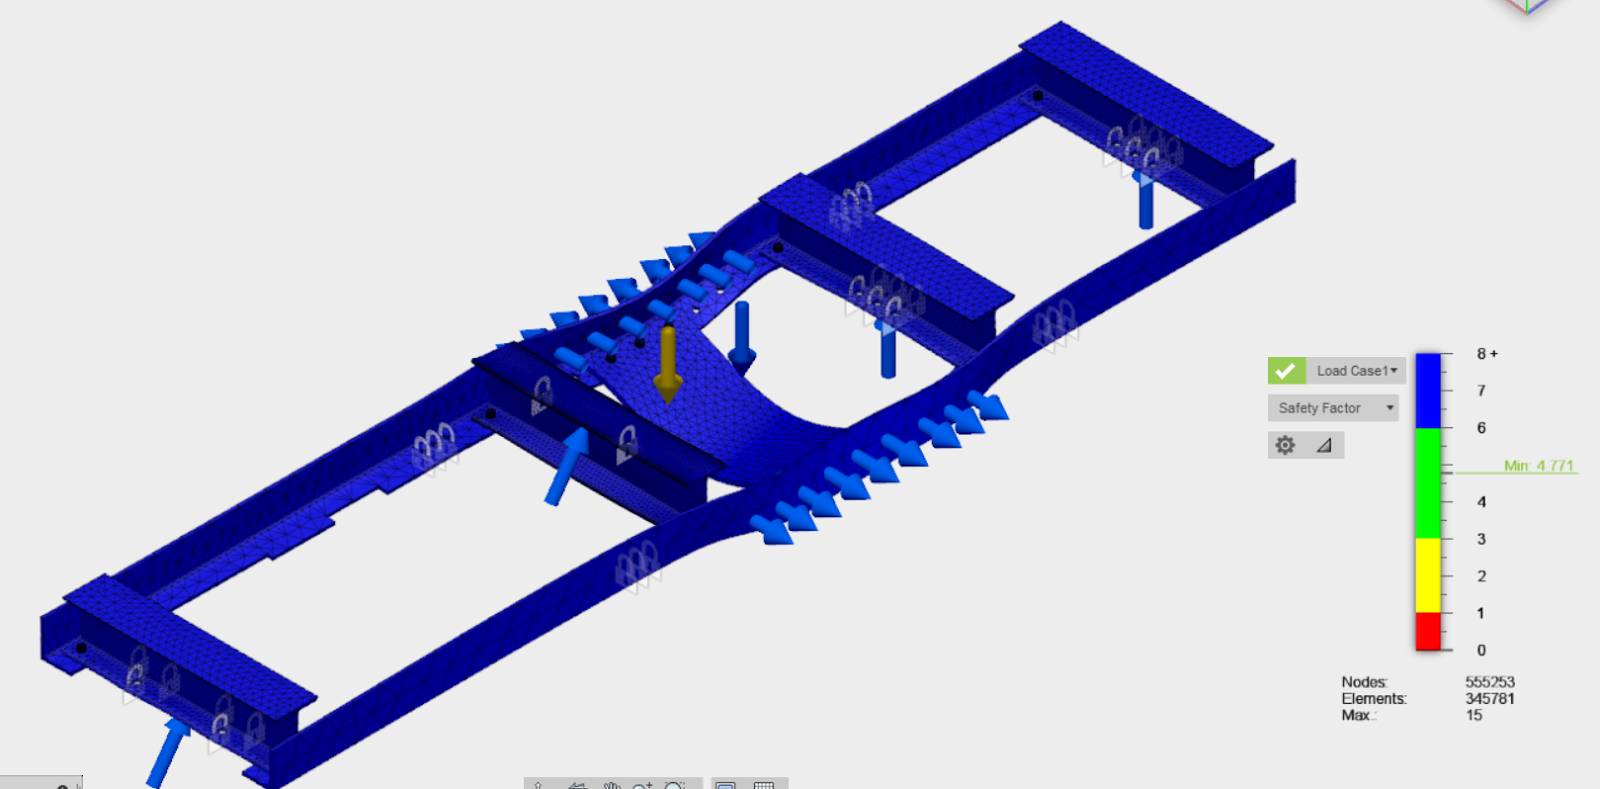
\includegraphics[width=\linewidth]{images/frame1}
        \caption{Frame Loading Case 1}
        \label{fig:frame1}
    \end{figure}
    \begin{figure}
        \centering
        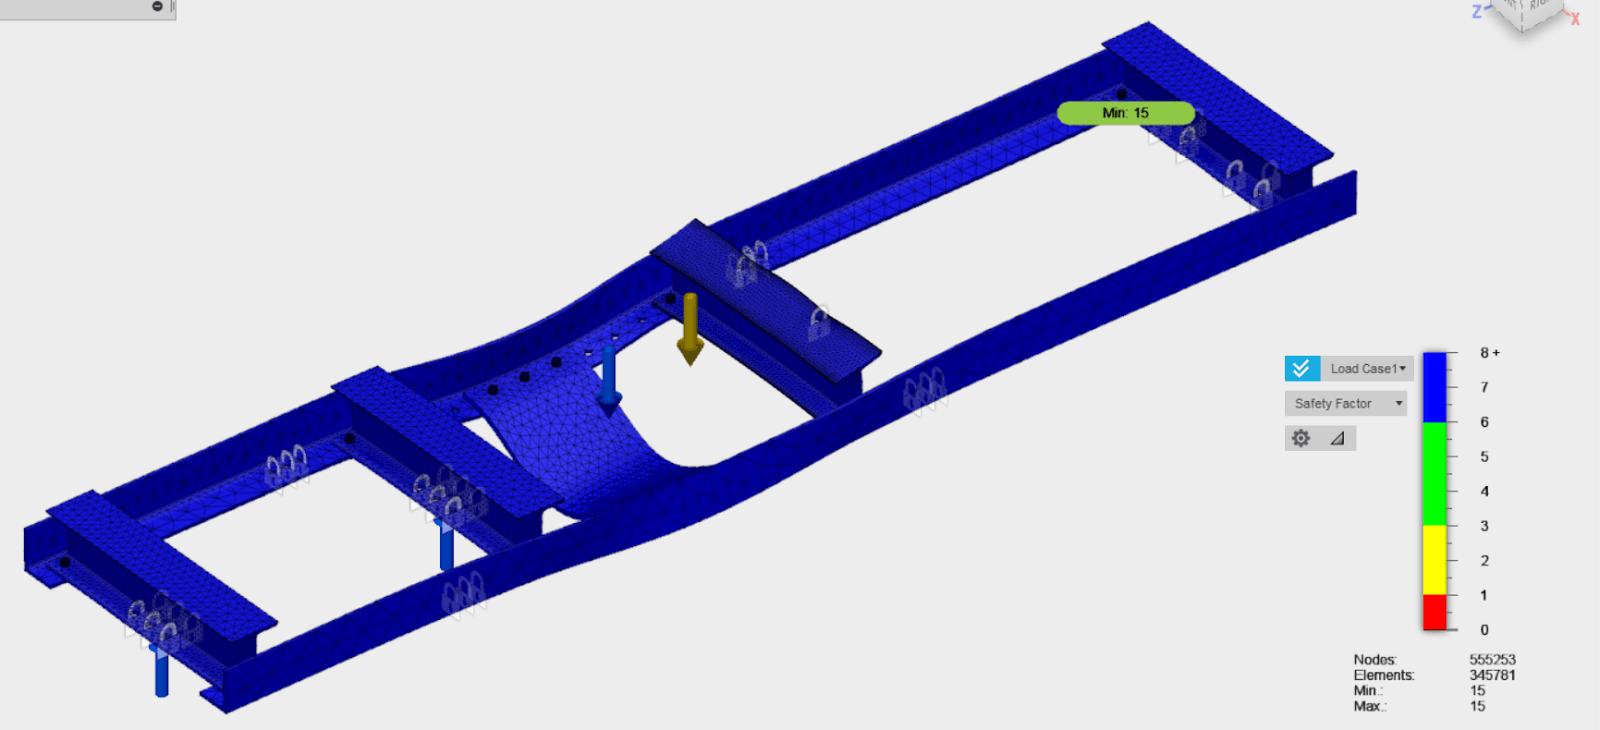
\includegraphics[width=\linewidth]{images/frame2}
        \caption{Frame Loading Case 2}
        \label{fig:frame2}
    \end{figure}
    \begin{figure}
        \centering
        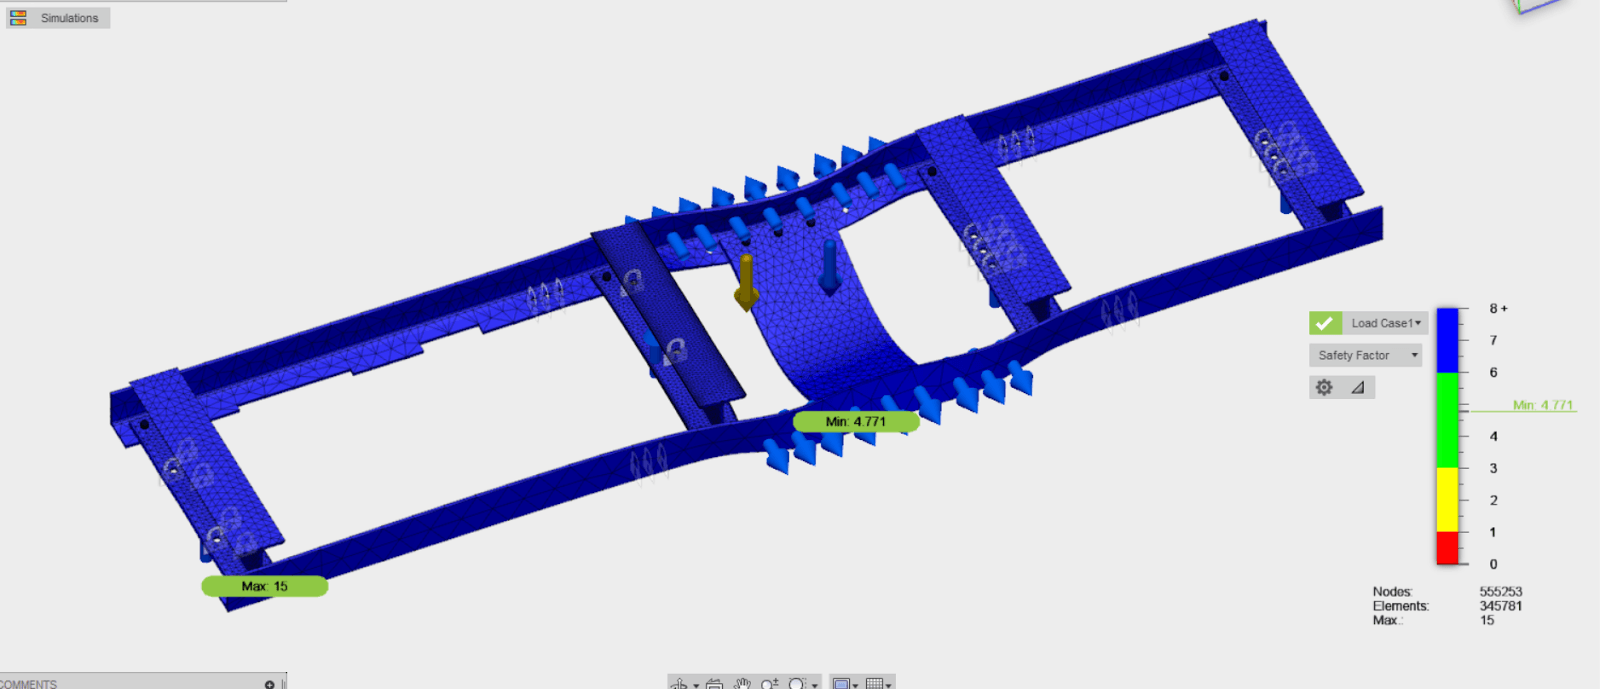
\includegraphics[width=\linewidth]{images/frame3}
        \caption{Frame Loading Case 3}
        \label{fig:frame3}
    \end{figure}
    \begin{itemize}
    \item The first loading scenario (\reffig{fig:frame1}) is a worst-case scenario in which the EC brakes actuate while friction drive is active. The lowest safety factor observed in the FEA model for this case is 4.176 on the bolts that the EC brakes would be attached to.
    \item The second loading scenario (\reffig{fig:frame2}) is where the friction drive system is active and providing forward propulsion to the pod. This case has a very high safety factor.
	\item The final loading case (\reffig{fig:frame3}) we will look at is when the friction drive is not running and the EC brakes are activated. The safety factor here is at 4.771, where the highest stress is on the bolts that the EC brakes are connected to.
	\item Pod structural design cases: at a minimum, this shall include initial acceleration, nominal deceleration, and a reasonably foreseeable off-nominal crash (FEA)
    \end{itemize}
\end{document}
